\section{Implementasi}
\label{sec:implementasi}

Tahap implementasi merupakan proses penerjemahan rancangan arsitektur dan kebutuhan fungsional ke dalam kode program yang berjalan. Pengembangan sistem MonPD Reborn dilakukan dengan menggunakan \emph{framework} ASP.NET Core MVC dan bahasa pemrograman C\#. Penulis berperan penuh dalam pembangunan \emph{Application Layer} (\emph{back-end}) dan \emph{Presentation Layer} (\emph{front-end}) untuk memastikan sistem dapat mengolah data perpajakan dari \emph{database} Oracle secara efisien.

\subsection{Alur Kerja Aplikasi}
\begin{figure}[H]
    \centering
    \begin{tikzpicture}[node distance=1.5cm]
        % Titik Mulai
        \node (start) [startstop] {User Mengakses Menu};
        
        % Tahap 1: Initial Load
        \node (step1) [process, below of=start] {\textbf{1. Pemuatan Kerangka}\\Memuat struktur HTML dasar (\emph{Razor View})};
        
        % Tahap 2: AJAX Request
        \node (step2) [process, below of=step1] {\textbf{2. Permintaan Data}\\Fungsi jQuery memicu \emph{AJAX Request} asinkron};
        
        % Tahap 3: Back-end Processing
        \node (step3) [process, below of=step2] {\textbf{3. Pengolahan Data}\\ \emph{Controller} memanggil \emph{Method} VM $\rightarrow$ Oracle via EF Core};
        
        % Tahap 4: Response
        \node (step4) [process, below of=step3] {\textbf{4. Pengembalian Hasil}\\Server mengirim data (\emph{JSON / Partial View})};
        
        % Tahap 5: Client-side Rendering
        \node (step5) [process, below of=step4] {\textbf{5. Perenderaan Dinamis}\\Data dirender ke DevExtreme DataGrid};

        % Garis Panah
        \draw [arrow] (start) -- (step1);
        \draw [arrow] (step1) -- (step2);
        \draw [arrow] (step2) -- (step3);
        \draw [arrow] (step3) -- (step4);
        \draw [arrow] (step4) -- (step5);
    \end{tikzpicture}
    \caption{Alur Komunikasi Data Asinkron MonPD Reborn}
    \label{fig:web_flow}
\end{figure}

Sistem MonPD Reborn dirancang untuk meminimalkan waktu tunggu pengguna melalui mekanisme pemuatan data asinkron. Berbeda dengan sistem lama yang memuat seluruh data secara sekaligus, alur kerja sistem ini dibagi menjadi beberapa tahapan sebagai berikut:
\begin{enumerate}
    \item \textbf{Pemuatan Kerangka (\emph{Initial Load})}: Saat pengguna mengakses menu, \emph{browser} hanya memuat struktur HTML dasar (\emph{Razor View}) tanpa data. Hal ini membuat halaman terasa instan saat dibuka.
    \item \textbf{Permintaan Data (\emph{AJAX Request})}: Setelah kerangka siap, fungsi JavaScript (jQuery) secara otomatis mengirimkan permintaan ke \emph{Action Method} di \emph{Controller} di latar belakang.
    \item \textbf{Pengolahan Data (\emph{Back-end Processing})}: \emph{Controller} memanggil \emph{method} statis di dalam \emph{ViewModel} yang kemudian bertugas melakukan kueri dan berinteraksi dengan \emph{database} Oracle melalui \emph{Entity Framework Core}.
    \item \textbf{Pengembalian Hasil (\emph{Response})}: Server mengembalikan data hasil olahan tersebut dalam format \emph{Partial View} atau JSON.
    \item \textbf{Perenderaan Dinamis (\emph{Client-side Rendering})}: Komponen DevExtreme DataGrid menerima data tersebut dan menampilkannya kepada pengguna tanpa perlu melakukan penyegaran halaman (\emph{refresh}).
\end{enumerate}

Mekanisme ini memungkinkan halaman terasa instan saat dibuka karena \emph{browser} tidak perlu menunggu seluruh data dari \emph{database} Oracle selesai ditarik sebelum menampilkan antarmuka.

\subsection{Pengembangan \emph{Application Layer} (\emph{Backend})}
Pada proyek ini, diterapkan pola arsitektur \emph{Fat ViewModel} dan \emph{Thin Controller}. Pendekatan ini bertujuan untuk memusatkan seluruh logika bisnis, pemfilteran, dan agregasi data di dalam \emph{ViewModel}, sehingga \emph{Controller} tetap ramping dan hanya berfungsi sebagai pengatur alur permintaan.

\begin{enumerate}
    \item \textbf{Pemetaan Entitas Data (Entity Mapping):} \\
    Sesuai dengan batasan masalah yang memfokuskan pengerjaan pada \emph{Application Layer}, penulis merancang kelas entitas yang merepresentasikan tabel fisik di server Oracle menggunakan \emph{Data Annotations} pada EF Core sebagaimana ditunjukkan pada Kode 4.1.

    \lstinputlisting[language={[Sharp]C}, caption={Pemetaan Entitas C\# ke Tabel Oracle pada Berkas TPemeriksaan.cs}]{program/TPemeriksaan.cs}

    Penjelasan Kode 4.1: Kode ini mendefinisikan hubungan antara properti di dalam kode aplikasi dengan kolom fisik di \emph{database} Bapenda. Penggunaan atribut \texttt{[Table("T\_PEMERIKSAAN")]} dan \texttt{[Column]} memastikan bahwa EF Core dapat melakukan kueri secara akurat ke tabel yang telah dioptimalkan oleh tim \emph{database} Bapenda. Properti dengan tipe data \emph{nullable} seperti \texttt{decimal?} pada \texttt{JumlahKb} digunakan untuk menangani kemungkinan data kosong di \emph{database} tanpa menyebabkan \emph{system crash}.

    \item \textbf{Struktur \emph{ViewModel} dan \emph{Controller}:} 
    Implementasi pola \emph{Thin Controller} ditunjukkan pada Kode 4.2, di mana \\ \texttt{PemeriksaanController} hanya bertugas menerima \emph{request}, melakukan instansiasi \emph{ViewModel}, dan mengembalikan \emph{Partial View}.
    
    \lstinputlisting[language={[Sharp]C}, caption={Implementasi \emph{Thin Controller} pada \texttt{PemeriksaanController.cs}}]{program/PemeriksaanController.cs}

    Penjelasan Kode 4.2: \emph{Action method} \texttt{Detail} menerima parameter \texttt{jenisPajak} dan \texttt{tahun}. Fungsi utama dari kode ini adalah memanggil kelas \emph{ViewModel} \texttt{Detail} dan menangani \emph{error handling} melalui blok \texttt{try-catch} untuk memastikan stabilitas aplikasi jika terjadi kegagalan sistem.

    \item \textbf{Logika Pengambilan Data (Fat ViewModel):} 
    Seluruh logika manipulasi data dipusatkan di dalam \\ \texttt{PemeriksaanVM.cs} seperti yang ditunjukkan pada Kode 4.3.
    
    \lstinputlisting[language={[Sharp]C}, caption={Logika Bisnis pada \emph{Fat ViewModel} \texttt{PemeriksaanVM.cs}}]{program/PemeriksaanVM.cs}

    Penjelasan Kode 4.3: Penulis menggunakan \emph{Entity Framework Core} untuk mengambil data dari tabel \texttt{TPemeriksaan}. Teknik optimasi kunci yang diterapkan adalah penggunaan \texttt{GroupBy} dan \texttt{ToDictionary} untuk melakukan pemetaan data \emph{master} objek pajak di dalam memori (\emph{in-memory mapping}). Hal ini dilakukan untuk menghindari operasi \emph{join} tabel yang berat di sisi \emph{database} Oracle, sehingga proses pencocokan nama Wajib Pajak berdasarkan NOP menjadi jauh lebih cepat.

    \item \textbf{Enkapsulasi Logika:} 
    Seluruh kalkulasi persentase pencapaian dan perbandingan target vs realisasi dilakukan di sisi \emph{server} sebelum dikirim ke \emph{front-end} guna menjaga konsistensi data dan meringankan beban komputasi di sisi \emph{client}.    

    \item \textbf{Implementasi AJAX (\emph{Frontend}):} 
    Untuk mengatasi masalah performa sistem lama, penulis mengimplementasikan fungsi asinkron menggunakan \emph{jQuery} sebagaimana ditunjukkan pada Kode 4.4.
    
    \lstinputlisting[language={JavaScript}, caption={Implementasi AJAX Request pada \texttt{PemeriksaanAJAX.js}}]{program/PemeriksaanAJAX.js}

    Penjelasan Kode 4.4: Fungsi \texttt{loadDetail} mengirimkan data permintaan ke \emph{Controller} di latar belakang. Penggunaan \texttt{beforeSend} berfungsi untuk menampilkan \emph{loading spinner} (\texttt{\#loading2-Detail}) sebagai indikator visual kepada pengguna bahwa data sedang diproses. Setelah data diterima (\emph{success}), hasilnya langsung dirender ke dalam elemen \texttt{\#Detail} tanpa perlu memuat ulang seluruh halaman web. Teknik ini berhasil mereduksi waktu muat secara drastis.
\end{enumerate}

\subsection{Pengembangan \emph{Presentation Layer} (\emph{Frontend})}
Pada \emph{Presentation Layer} (\emph{Frontend}), penulis fokus pada pembangunan antarmuka yang responsif dan interaktif menggunakan jQuery dan \emph{toolkit} DevExtreme.
\begin{enumerate}
    \item \textbf{Implementasi AJAX:} Penulis menulis fungsi \emph{JavaScript} seperti \texttt{fnShow()} untuk memicu pemuatan tabel secara asinkron. Teknik ini berhasil mereduksi waktu muat dari $\pm 120$ detik menjadi hanya $\pm 3 - 5$ detik.
    \item \textbf{Konfigurasi \emph{DevExtreme DataGrid}:} Komponen ini dikonfigurasi untuk menangani volume data besar dengan fitur \emph{server-side paging}. Penulis juga mengimplementasikan \emph{Banded Columns} untuk mengelompokkan data yang berkaitan, seperti kolom ``Pokok'' dan ``Sanksi'' di bawah kategori tahun yang sama.
    \item \textbf{Fitur \emph{Drill-down}:} Melalui fungsi \texttt{showDetailModal()}, pengguna dapat mengklik angka pada tabel rekapitulasi untuk menampilkan \emph{pop-up} detail transaksi individual yang dimuat melalui \emph{Partial View} \texttt{\_Detail.cshtml}.
\end{enumerate}


\subsection{Hasil Implementasi Fitur Utama}
Berikut adalah hasil dari implementasi kode program yang telah dilakukan:
\begin{itemize}
    \item Dashboard Analitik Utama: \\
    Tampilan pusat komando yang menyajikan KPI (\emph{Key Performance Indicator}) secara instan untuk setiap jenis pajak ditunjukkan pada gambar \ref{fig:dashboard-utama-monpd}.
    \begin{figure}[H]
        \centering
        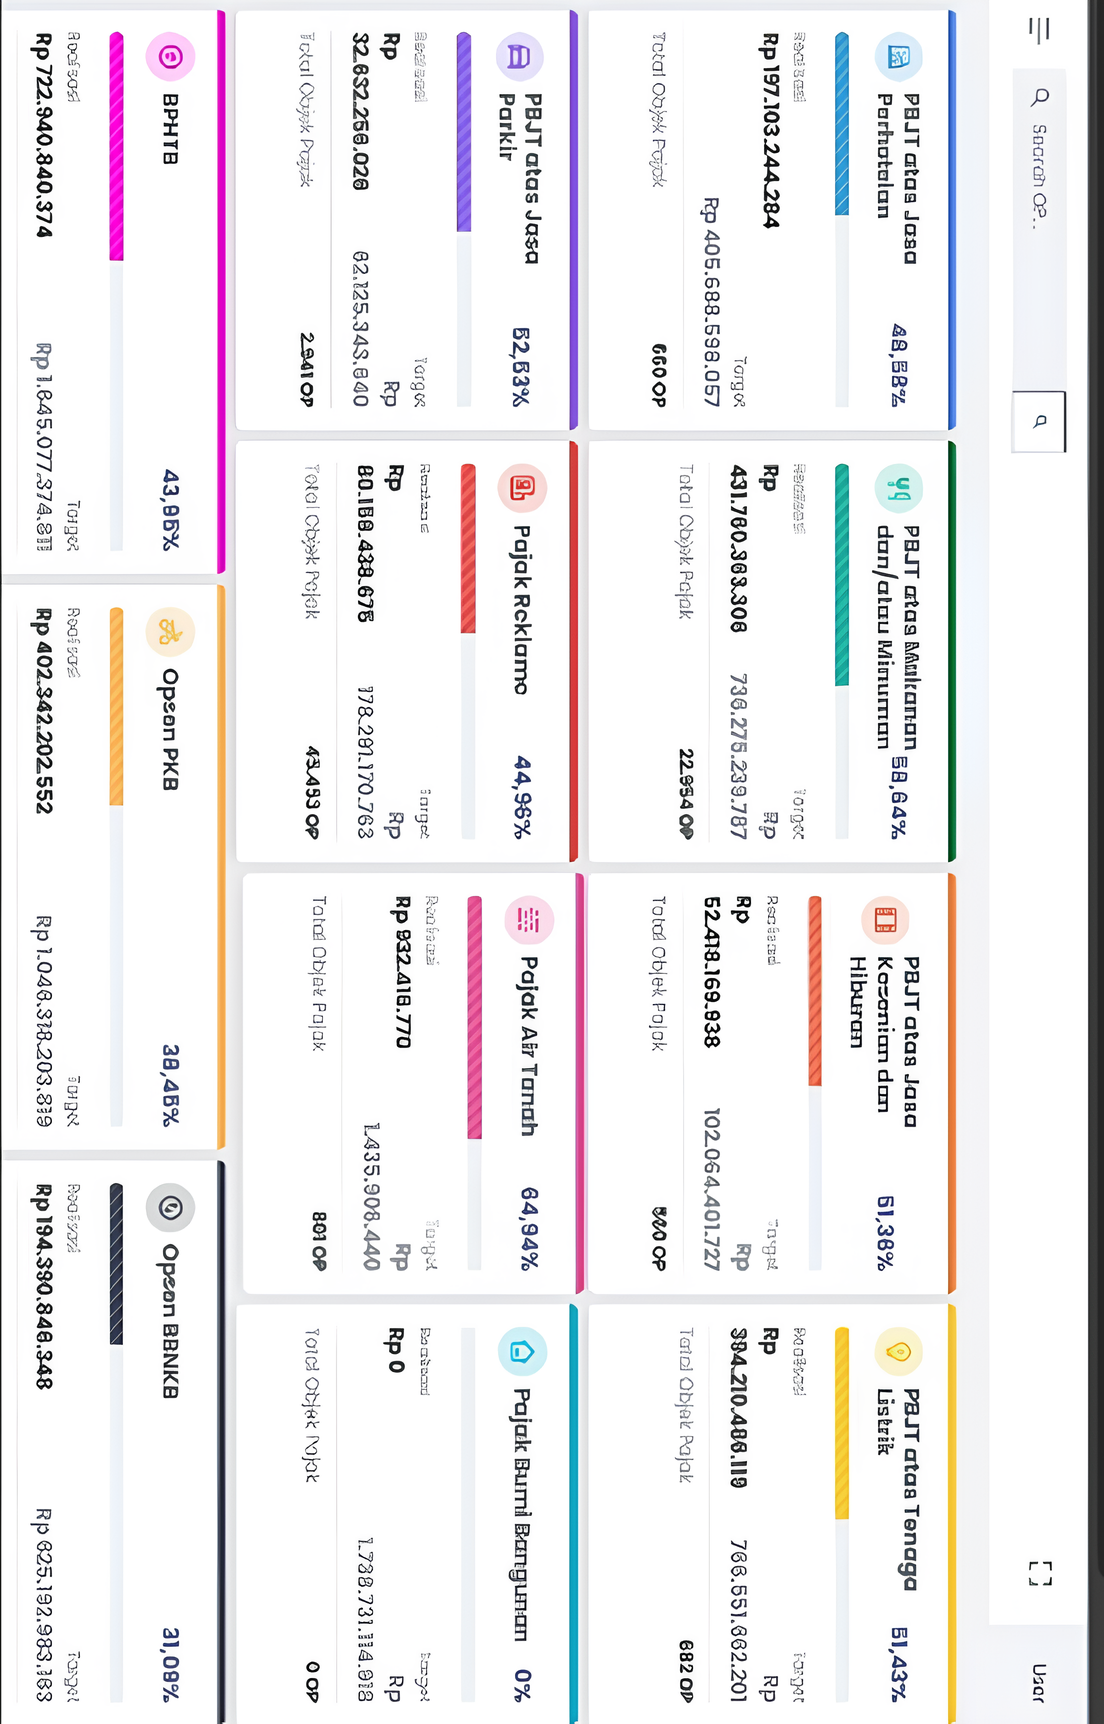
\includegraphics[width=0.95\textwidth]{gambar/dashboard-utama-monpd.png}
        \caption{Tampilan \emph{Dashboard} Utama MonPD Reborn}
        \label{fig:dashboard-utama-monpd}
    \end{figure}

    \item Template Modul Analitik: \\
    Standar tampilan yang memisahkan antara panel filter, ringkasan KPI, dan tabel rincian diimplementasikan pada seluruh modul, seperti yang terlihat pada gambar \ref{fig:dashboard-menu-monpd}.
    \begin{figure}[H]
        \centering
        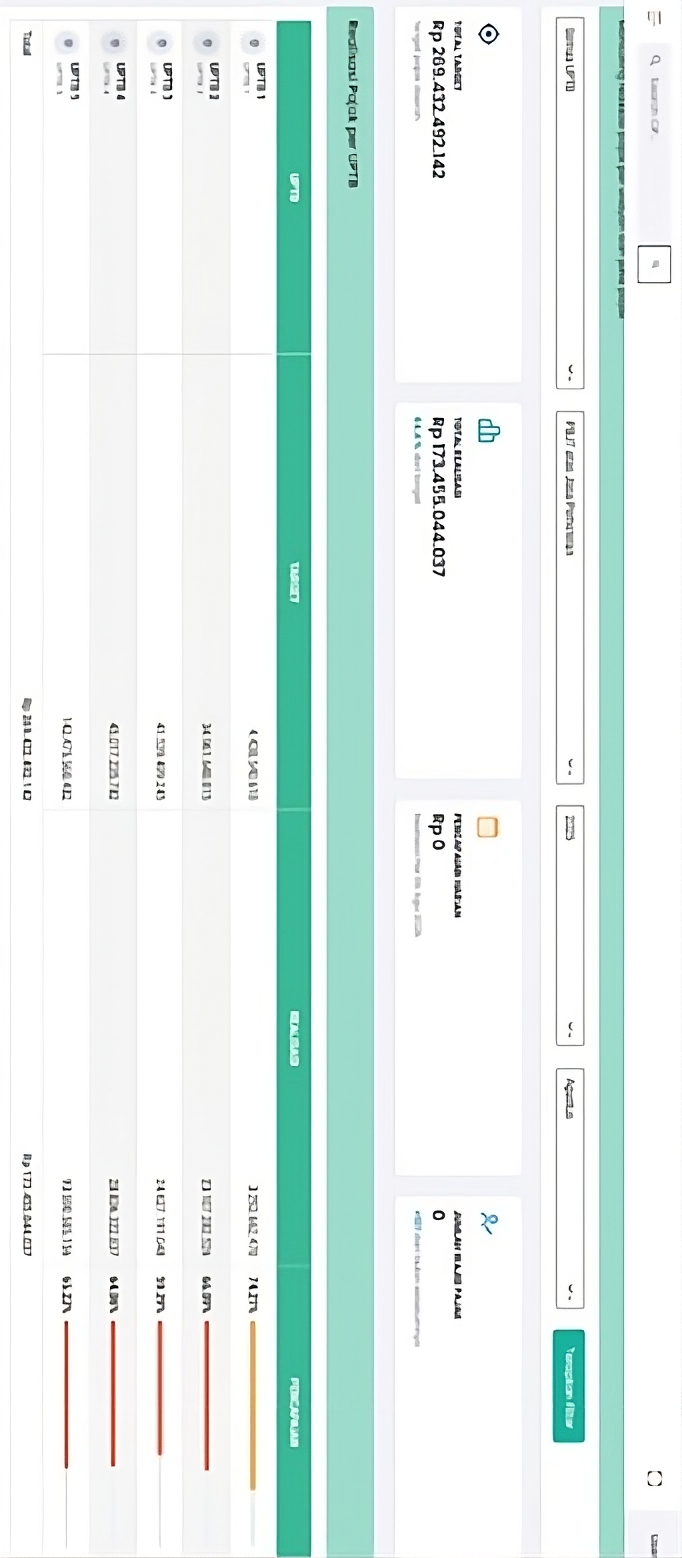
\includegraphics[width=0.55\textwidth]{gambar/dashboard-menu-monpd.png}
        \caption{Tampilan \emph{Dashboard} Menu MonPD Reborn}
        \label{fig:dashboard-menu-monpd}
    \end{figure}

    \item Interaktivitas Data: \\
    Fitur filter per kolom, pencarian instan, dan pengurutan data pada komponen DataGrid ditunjukkan pada gambar \ref{fig:datagrid}.
    \begin{figure}[H]
        \centering
        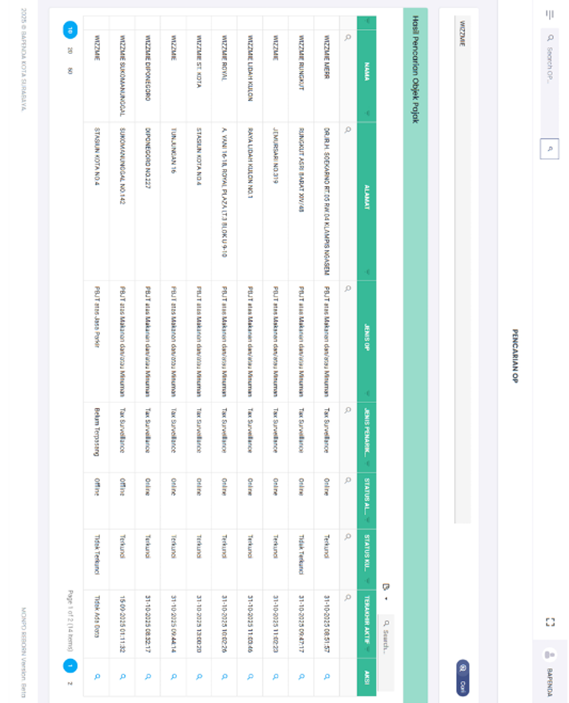
\includegraphics[width=0.99\textwidth]{gambar/datagrid.png}
        \caption{Implementasi DevExtreme DataGrid dengan Fitur Interaktif}
        \label{fig:datagrid}
    \end{figure}

    \item Detail \emph{Pop-up} (\emph{Drill-down}): \\
    Mekanisme pemuatan data detail tanpa kehilangan konteks halaman utama menggunakan modal asinkron ditunjukkan pada gambar \ref{fig:popup-detail}.
    \begin{figure}[H]
        \centering
        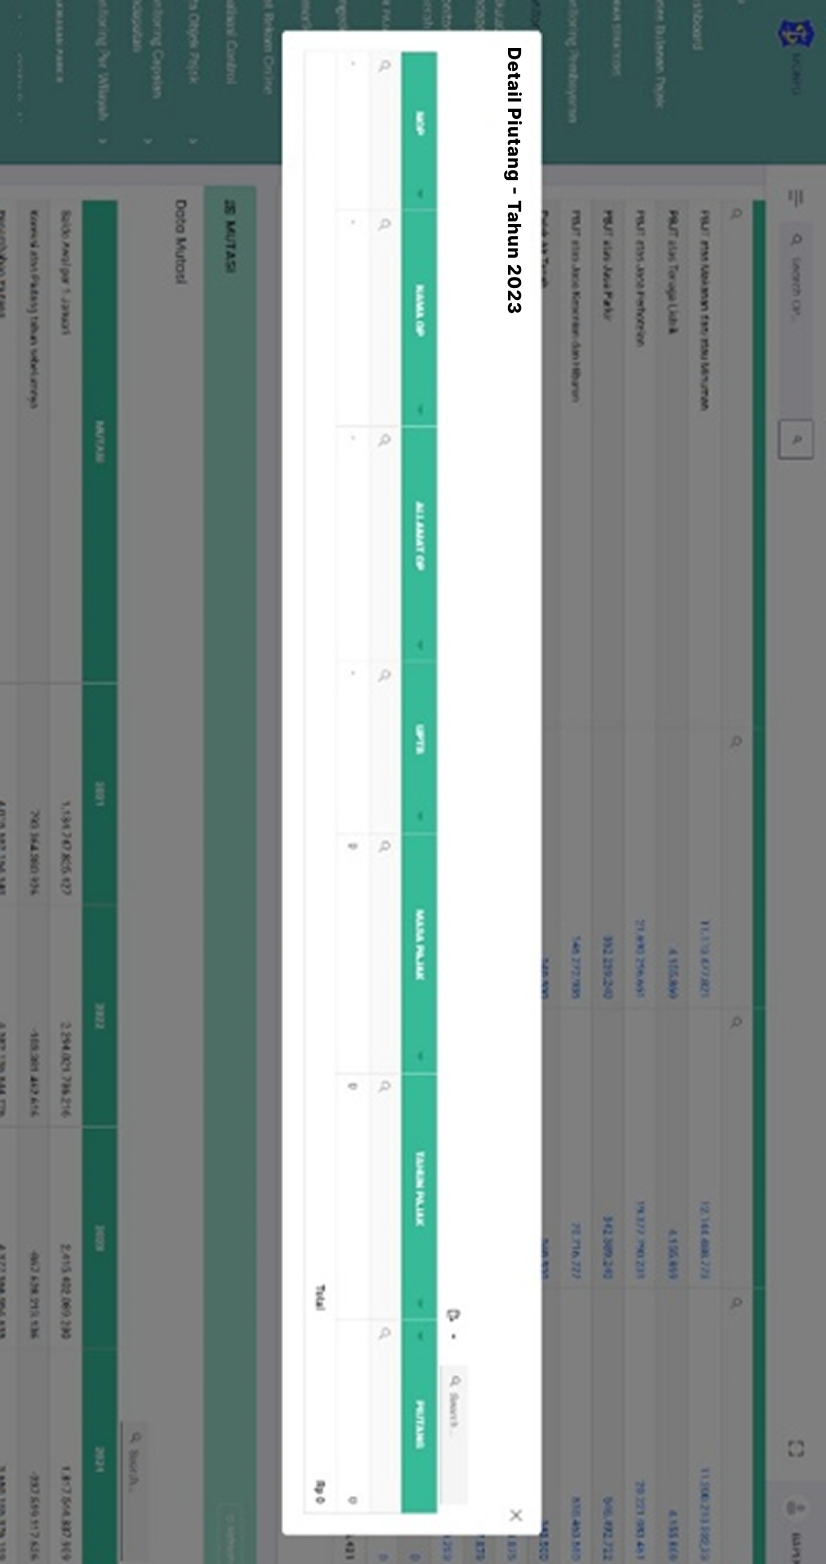
\includegraphics[width=0.67\textwidth]{gambar/popup-detail.png}
        \caption{Implementasi Detail \emph{Pop-up} pada MonPD Reborn}
        \label{fig:popup-detail}
    \end{figure}

    \item Visualisasi Geospasial: \\
    Plot lokasi objek pajak di atas peta Kota Surabaya untuk analisis potensi kewilayahan ditunjukkan pada gambar \ref{fig:geospasial}.
    \begin{figure}[H]
        \centering
        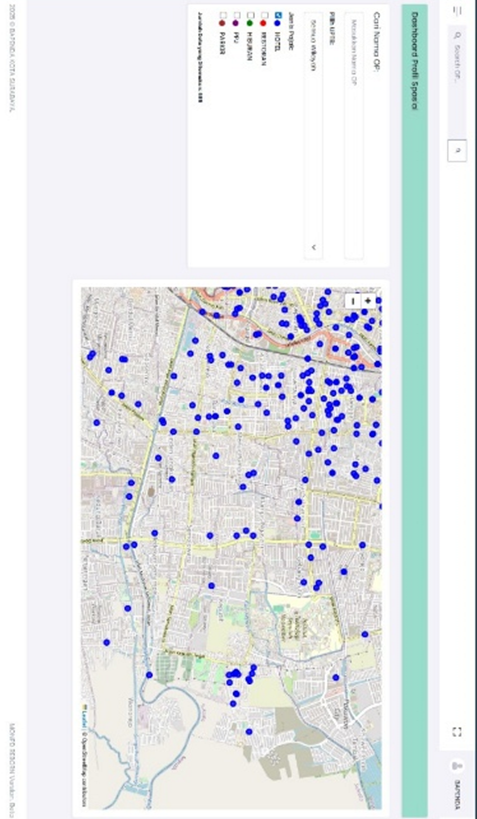
\includegraphics[width=0.76\textwidth]{gambar/geospasial.png}
        \caption{Visualisasi Geospasial pada MonPD Reborn}
        \label{fig:geospasial}
    \end{figure}

    \item Tabel Rekapitulasi Kinerja: \\
    Penyajian perbandingan target dan realisasi yang dilengkapi dengan \emph{progress bar} otomatis ditunjukkan pada gambar \ref{fig:realisasi-pajak}.
    \begin{figure}[H]
        \centering
        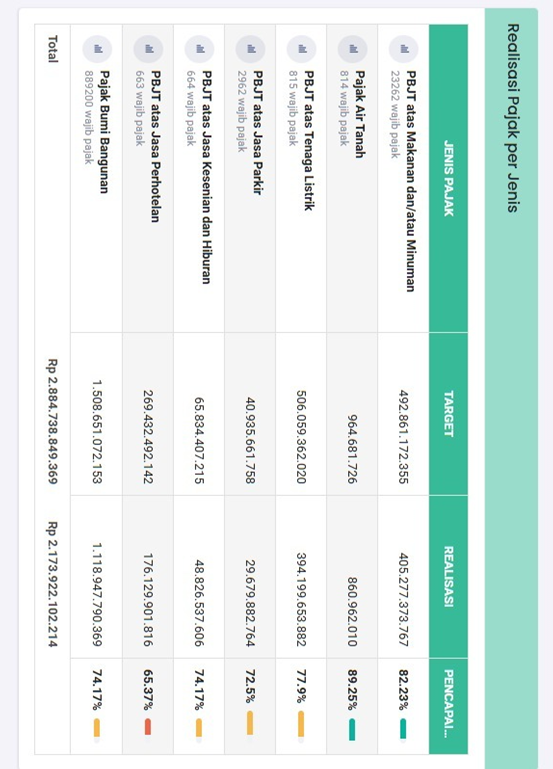
\includegraphics[width=0.93\textwidth]{gambar/realisasi-pajak.png}
        \caption{Tabel Realisasi Pajak}
        \label{fig:realisasi-pajak}
    \end{figure}

\end{itemize}
